\subsection{Shared Space træk i Nytorv/Østerågade området}
\label{omrade_sharedspace}
For at få en forståelse af hvordan trafikanterne færdes i Nytorv/Østerågade området, er det vigtigt først at fastlægge, hvilken type område det er. Området har mange træk fra Shared Space, og derfor er det relevant at sammenligne området med dette begreb.
Tit og ofte anvender man Shared Space i områder, hvor der er et kryds, eller hvor der er et sammenhængende område, for at skabe en slags balance mellem de forskellige trafikantgrupper. (Vejregler, 2013)

\begin{figure}[htbp]
   \centering
   \begin{adjustbox}{max width=\textwidth}
     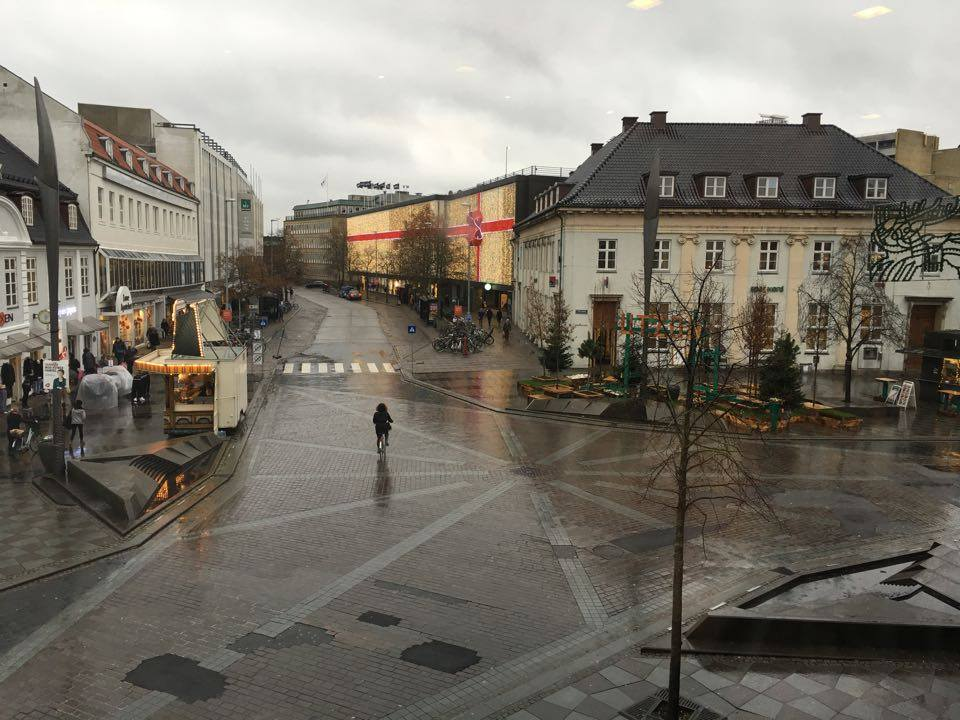
\includegraphics[scale=0.3]{figures/Billederogfigur/Nytorvoverblik.jpg}
  \end{adjustbox}
   \caption{Oveblik over Nytorv}
   \label{fig:nytorv}
 \end{figure}

Med en balance menes der, at et af formålene med et Shared Space er at ingen af trafikantgrupperne vægtes højere end andre trafikantgrupper. På den måde vil man ikke bryde et sammenhængende område, da man forsøger at kombinere hele områdets funktioner i et. Netop dette princip kan man tydeligt fornemme nede ved Nytorv/Østerågade området.  På figur ~\cref{fig:nytorv} side \pageref*{fig:nytorv} 1 kan man se, at området består af et T-kryds, hvor der rundt om er placeret mange shopping faciliteter og caféer. Desuden forbinder området de to gågader, som gør området til et sammenhængende område. Kriterierne for et område, hvor Shared Space kan benyttes, er altså her opfyldt.
Det er tydeligt, at belægningerne, både på fortov og vej, er meget lig udeseende, hvilket er typisk for et Shared Space område. Der er heller ikke meget afmærkning i form af cykelstier eller kørebaner, som ville have haft til formål at lede trafikanterne. Skiltning, er heller ikke meget brugt og typisk ser man kun et ”E49-, E51- eller E53-skilt” i Shared Space områder, som enten fortæller, om det er en gågade, opholds- og legeområde, eller en fartdæmpet zone, hvor makshastigheden typisk må være 20-30 km/t.  Rundt om Nytorv/Østerågade området, er der skiltet med E53-skilte, hvor der er en tilladt makshastighed på 30 km/t. Det kan ses på figur \cref{fig:Skiltning} side \pageref{fig:Skiltning}, som er taget ved Adelgade, lige inden man kommer ind i Nytorv/Østerågade området.

\begin{figure}[htbp]
   \centering
   \begin{adjustbox}{max width=\textwidth}
     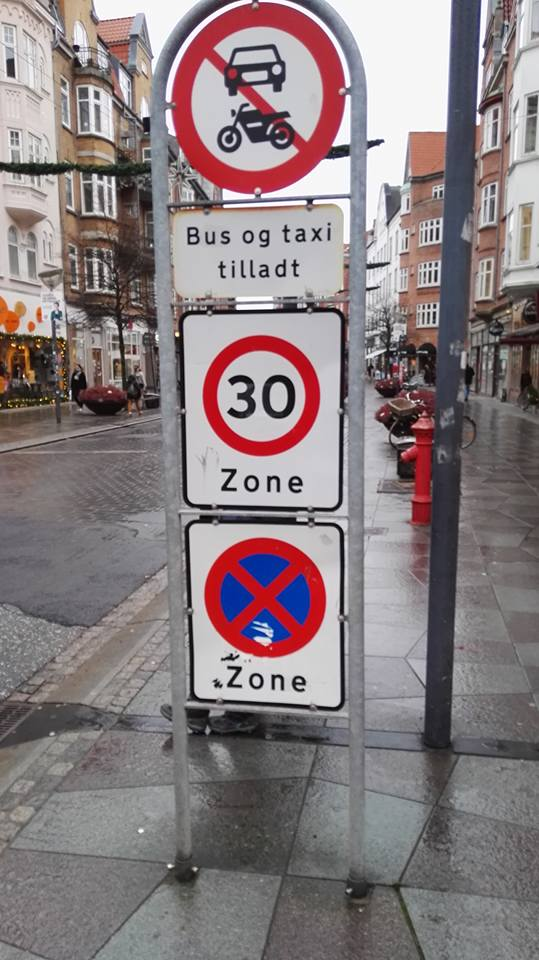
\includegraphics[scale=0.2]{figures/Billederogfigur/skiltning.jpg}
  \end{adjustbox}
   \caption{Skiltning rundt om området}
   \label{fig:Skiltning}
 \end{figure}

I området er der dog en del bustrafik, hvilket strider imod Shared Space’ principper. Det kan give problemer for busserne, at overholde tidsplanerne, da de ofte vil være nødsaget til, at skulle holde tilbage for de mange passerende fodgængere. Det vil derved mindske effektiviteten af den kollektive trafik. Dog er der oftest i ruteplanerne taget højde for en sådan forsinkelse, og på korte strækninger vil indflydelsen kunne tænkes at være begrænset. Busserne kræver nogle busstoppesteder, for at passagerer kan stige af og på busserne i området.

\begin{figure}[htbp]
   \centering
   \begin{adjustbox}{max width=\textwidth}
     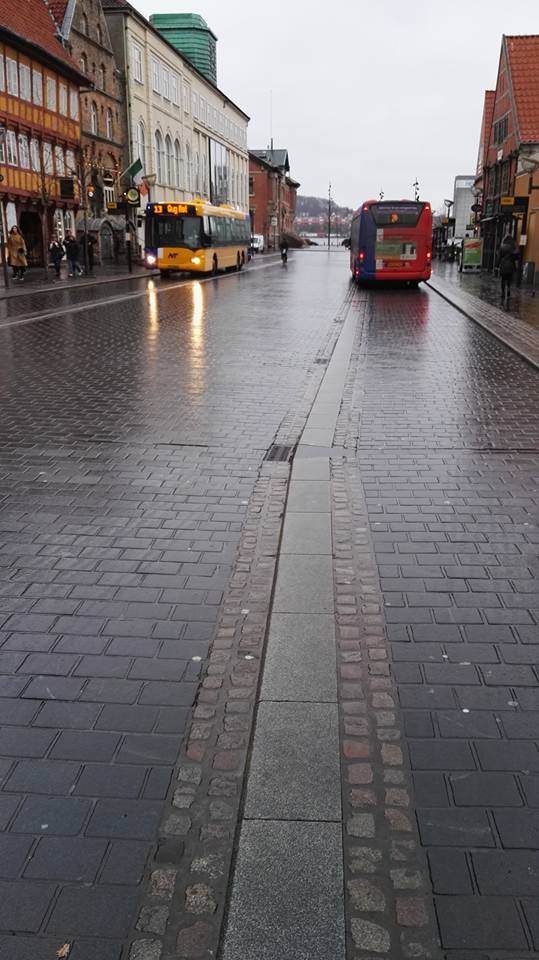
\includegraphics[scale=0.2]{figures/Billederogfigur/Busstoppesteder.jpg}
  \end{adjustbox}
   \caption{De to busstoppesteder}
    \label{fig:Busstoppesteder}
 \end{figure}

På figur \cref{fig:Busstoppesteder} side \pageref{fig:Busstoppesteder} kan man se de to etablerede busstoppesteder, som er placeret lige efter, hvor Bispensgade udmunder ved Østerågade. Placeringen af bustoppestederne er lige udenfor det mest befærdede område, som strækker sig mellem de to gågader og ned ad Nytorv. Det er medvirke til, at det skaber mindst mulige trafikale problemer.
I et Shared Space område kræves også mange holdepladser til cykler. På Nytorv er der på begge sider af vejen et forholdsvist bredt fortov, som har til formål, at skabe en masse plads, hvor cyklerne kan holde parkeret. Det er en nødvendighed, da der færdes mange cykler i området, og for at de mange cyklister skal kunne benytte sig af de mange shopping faciliteter, kræves der altså nogle holdesteder.
Der er altså rigtigt mange træk, som man i området kan observere, minder meget om et Shared Space’ princip, og projektet vil i det næste afsnit undersøge, hvordan området bliver benyttet.


\subsection{Trafikanternes benyttelse af Nytorv som et Shared Space}
\label{benyttelse_omrade}
I området er der meget få retningslinjer og afmærkninger til at lede trafikanterne, hvis stort set ingen. På \cref{fig:Fodfelt} side \pageref{fig:Fodfelt} kan man se en af de to fodgængerfelter, som er i området. Det er på billedet let nok at se afmærkningerne, da billedet er taget fra et fugleperspektiv.

\begin{figure}[htbp]
   \centering
   \begin{adjustbox}{max width=\textwidth}
     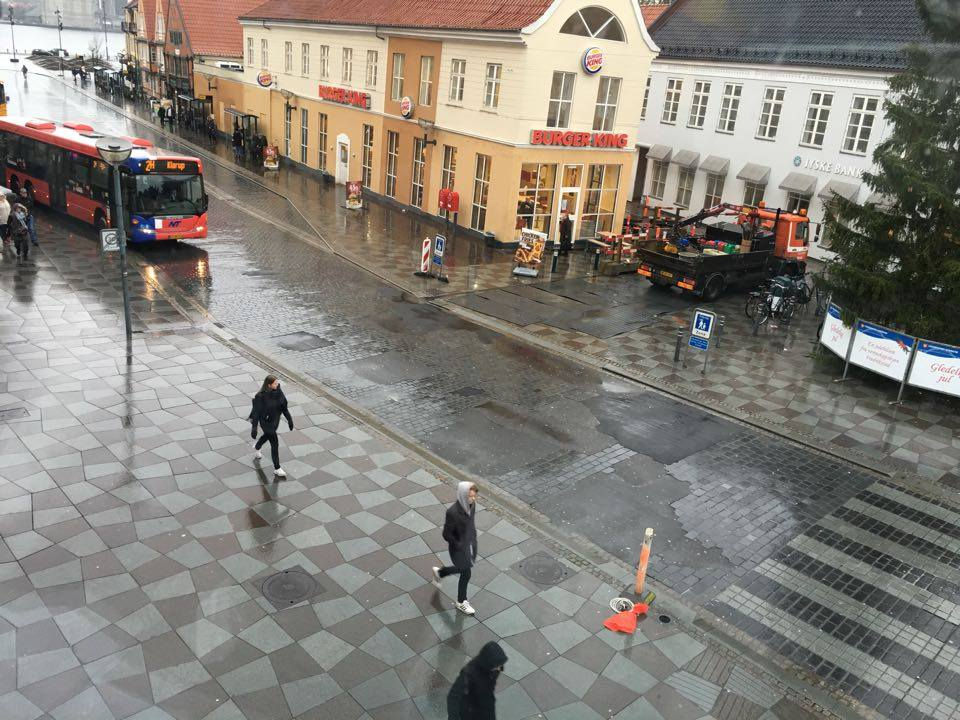
\includegraphics[scale=0.3]{figures/Billederogfigur/Fodfelt.jpg}
  \end{adjustbox}
   \caption{Fodgængeroverfeltet}
   \label{fig:Fodfelt}
 \end{figure}

Men en observation af dette område kan bekræfte, at det kan være svært for cyklisterne at se fodgængerfeltet, når de kommer cyklende mod det. . Det er især cyklister, som kommer rundt svinget fra Nytorv mod havnen. Det er blandt andet også denne hypotese, at interviewsene senere i rapporten tager lidt udgangspunkt i, hvor trygheden for de passerende fodgængere undersøges.
Det er her spørgsmålet kommer ind i billedet, om flere retningslinjer vil skabe mere tryghed. Det er i hvert fald tydeligt, at der er blevet formået at binde området sammen set fra de bløde trafikanters perspektiv. Udelukkelsen af biler har tydeligt præget fordelingen af trafikantgrupper i området, og langt størstedelen er fodgængere og cyklister (tabel over trafiktælling).
En vurdering af området tyder på, at den indbyrdes respekt overfor hinanden, mellem de forskellige trafikantgrupper, ikke er pålagt af området, men individet selv, netop fordi, at området ikke pålægger det. Shared Space har altså en form for psykologisk effekt, som får trafikanterne til at være opmærksomme på hinanden, og hjælpe hinanden gennem området bedst muligt. Dog er dette ikke et argument for et trygt område at færdes i. Kvalitative interviews vil her være en god måde at undersøge på, om især fodgængerne føler sig trygge, ved at passere området.
I det næste afsnit vil der blive undersøgt via kvalitative interviews, om fodgængerne føler sig trygge overfor cyklisterne, busserne og bilerne, når de passere fodgængeroverfeltet. Herved også for at få en forståelse af, om området føles trygt, og om de Shared Space træk der er i området, skaber trafikale problemer eller ej.
